\documentclass{article}
\usepackage[utf8]{inputenc}
\usepackage{graphicx}

\title{Esperienza di Millikan}
\author{Francesco Pio Merafina, Onofrio Davide Caputo, Alessandro Lamesta}
\date{}

\begin{document}
\maketitle
\section{Abstract:}
L'esperienza svolta in laboratorio è una replica dell'esperienza di Millikan per misurare il valore della carica elettrica dell'elettrone in Coulomb mediante la ionizzazione di particelle di olio.
~
\section{Cenni teorici:}
Per verificare se effettivamente la carica elettrica di un oggetto è sempre un multiplo intero di un valore fondamentale si sfruttano i campi elettrici; infatti dopo la ionizzazione delle particelle di olio esse sono sensibili ai campi elettrici, quindi misurando tempi di caduta libera e di risalita, ottenuta mediante applicazioni di un campo elettrico, si sono ottenuti i risultati.
~
\section{Apparato sperimentale:}
L'apparato utilizzato consiste in un cilindro nel quale sono presenti due piastre che rappresentano le armature di un condensatore con campo elettrico regolabile tra due valori in modulo (700 Vcm$^{-1}$) uguale ma segni opposti ed un valore di campo elettrico nullo, una sorgente di radiazioni $\alpha$, un nebulizzatore per spruzzare l'olio, un sistema di illuminazione e di ottica che proiettano su uno schermo il contenuto del cilindro, un cronometro digitale per misurare i tempi di salita e di discesa della goccia, una griglia per osservare la distanza percorsa dalla goccia.
~
\section{Metodologia di misura:}
Prima di eseguire l'esperimento si è provveduto a pulire il cilindro dove andranno spruzzate le goccioline d'olio, in modo da rimuovere i residui dovuti a precedenti esperimenti. Dopo questa operazione si è proceduto nella messa a fuoco della camera mediante la strumentazione ottica e l'illuminazione; successivamente si è nebulizzando l'olio nel cilindro, e si è attivata la sorgente di radiazioni $\alpha$ per ionizzare le particelle di olio. La distanza, fissa per tutte le goccioline di olio, scelta per la misura dei tempi di salita e discesa è di 1mm con incertezza uguale alla minima partizione della griglia. Una volta scelta la goccia si è provveduto a misurare i tempi di discesa con campo elettrico spento, e di risalita con campo elettrico acceso. Una nota a margine va fatta per le gocce misurate, a causa di alcuni problemi legati all'apparecchiatura molte gocce sono state perse durante le prime misure rendendo difficoltoso il procedimento.
~
\section{Analisi dati:}
Le formule di riferimento teorico sono le seguenti per le due situazioni:
\subsection{Discesa:}
equazione delle forze:
\begin{equation}
    F=F_{Peso}-F_{viscosità}=\frac{4\pi r^3 \rho g}{3}-\frac{6\pi r \eta_0 v_0}{1+\frac{b}{pr}}=0
\end{equation}
Raggio goccia d'olio:
\begin{equation}
    r=-\frac{b}{2p}+((\frac{b}{2p})^2+\frac{9 \eta_0 v_0}{2g\rho})^\frac{1}{2}
\end{equation}
Al posto del "$+$" ci dovrebbe essere un "$\pm$" ma la soluzione negativa non ha fisicamente senso.
\subsection{Salita:}
Valore carica elettrica:
\begin{equation}
    q=\frac{4dr^3g\pi\rho}{3}(1+\frac{v_r}{v_0})
\end{equation}
~
\section{Risutati e conclusioni:}
Osservando i dati delle gocce d'olio:
\begin{itemize}
    \item goccia 1: raggio=(329.87$\pm$11.70)nm, carica=(5.40$\pm$6.89)10$^{-19}$C
    \item goccia 2: raggio=(854.84$\pm$24.65)nm, carica=(7.40$\pm$0.72)10$^{-19}$C
    \item goccia 3: raggio=(402.22$\pm$15.55)nm, carica=(3.63$\pm$1.84)10$^{-19}$C
    \item goccia 4: raggio=(453.61$\pm$13.50)nm, carica=(5.74$\pm$1.82)10$^{-19}$C
    \item goccia 5: raggio=(414.60$\pm$24.37)nm, carica=(6.61$\pm$10.63)10$^{-19}$C
\end{itemize}
Possiamo concludere che, tenendo conto delle grandi incertezze sui valori di carica, questi valori siano compatibili con dei multipli interi della carica fondamentale 1.60*10$^{-19}$ C.
~
\section{Grafici e tabelle:}
\begin{figure}[h!]
    \centering
    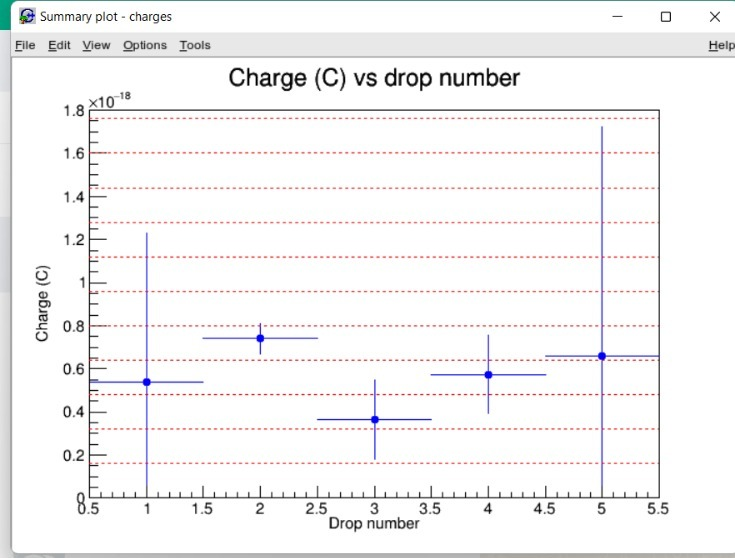
\includegraphics[width=\linewidth]{WhatsApp Image 2022-07-15 at 21.02.47.jpeg}
    \caption{Distribuzione dei valori di carica sulle gocce d'olio}
    \label{figura1}
\end{figure}
\begin{figure}[h!]
    \centering
    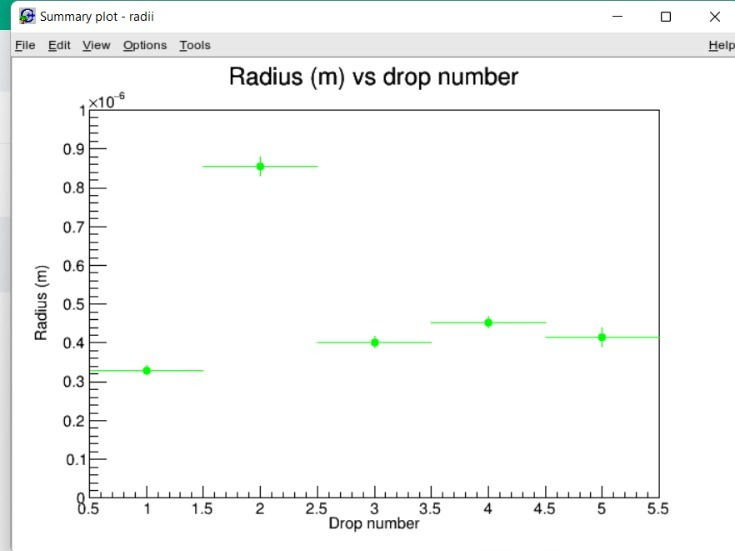
\includegraphics[width=\linewidth]{WhatsApp Image 2022-07-15 at 21.03.04.jpeg}
    \caption{Distribuzione dei raggi delle gocce d'olio}
    \label{figura1}
\end{figure}









\end{document}